\documentclass{article}
\usepackage[margin=1in]{geometry}
\usepackage[utf8]{inputenc}
\usepackage{hyperref}
\usepackage{courier}
\usepackage{textcomp}
\usepackage{indentfirst}
\usepackage{graphicx}

\title{SMDO group's git and GitHub workflow}
\author{Yicong Fu}
\date{September 2021}

\begin{document}

\maketitle

\section{Introduction: git and GitHub}

\subsection{Git}
Git is the version control software the group use to streamline the development of all our research code.
There are two main ingredients of git: repository and local copy.
Repository is the public place where everyone gets the code from and uploads the changes to.
Local copy is like a scratch space for you to play around with the code, develop on certain feature and test
in whatever way you want to.
Once you feel comfortable with the changes you've made locally, you could upload those changes to the
repository such that everyone else can get on the same page by updating their local copy using the latest repository.

Basic git only has command line interface (CLI).
If you need a GUI you could download GitHub Desktop.
In terms of how git works and how to use git CLI, there are many good references out there. The following ones are my favorite beginning-level tutorials:

\begin{itemize}
    \item \href{https://missing.csail.mit.edu/2020/version-control/}{https://missing.csail.mit.edu/2020/version-control/}
    \item \href{https://learngitbranching.js.org/}{https://learngitbranching.js.org/}
\end{itemize}

\subsection{GitHub}

Technically, git repositories can be hosted either on local machine, on some server in the local network, or
on the internet.
GitHub is one of the biggest service provider of internet hosting for git repositories.
There are two main versions of GitHub: public (github.com) and enterprise (for us it's github.gatech.edu).
They are separate from each other, so you will need different accounts.
In the past we use both: we kept ongoing development privately on GaTech GitHub, and periodically
released stable versions to public GitHub.
But now we will use public GitHub only.
The following sections will cover the new workflow.

\section{Workflow}

\subsection{Prerequisites}

First, make sure you have an account for public github and git on your local machine,
which is usually preinstalled on Unix-like systems (but not for Windows).

Next, register this account on your local machine to let git know who you are.
This can be done by running the following commands in terminal from anywhere:

\texttt{git config --global user.name your-account-name}

\texttt{git config --global user.email your-account-email}

The commands above will write account information to your global git configuration file, which is in \texttt{\$HOME/.gitconfig}
for Linux and MacOS.
Notice that if you also have other projects under a different github account (e.g. another github.com account
or github.gatech.edu account), you will need to set it up separately by running the following
commands in the project folder in terminal:

\texttt{git config user.name your-account-name}

\texttt{git config user.email your-account-email}

The commands above essentially write to a repo specific configuration file \texttt{project-folder/.git/config}.

Another thing you'll need to do is to run:

\texttt{git config --global pull.ff only}

This will prevent some issues when pulling.

\subsection{The [fork]-[develop]-[pull request] work flow}

Using this workflow, everyone will have a ``forked'' repository under their own GitHub account,
write and push the code to this repo, and finally update the group's repo via ``pull request''.

\begin{figure}[h]
    \centering
    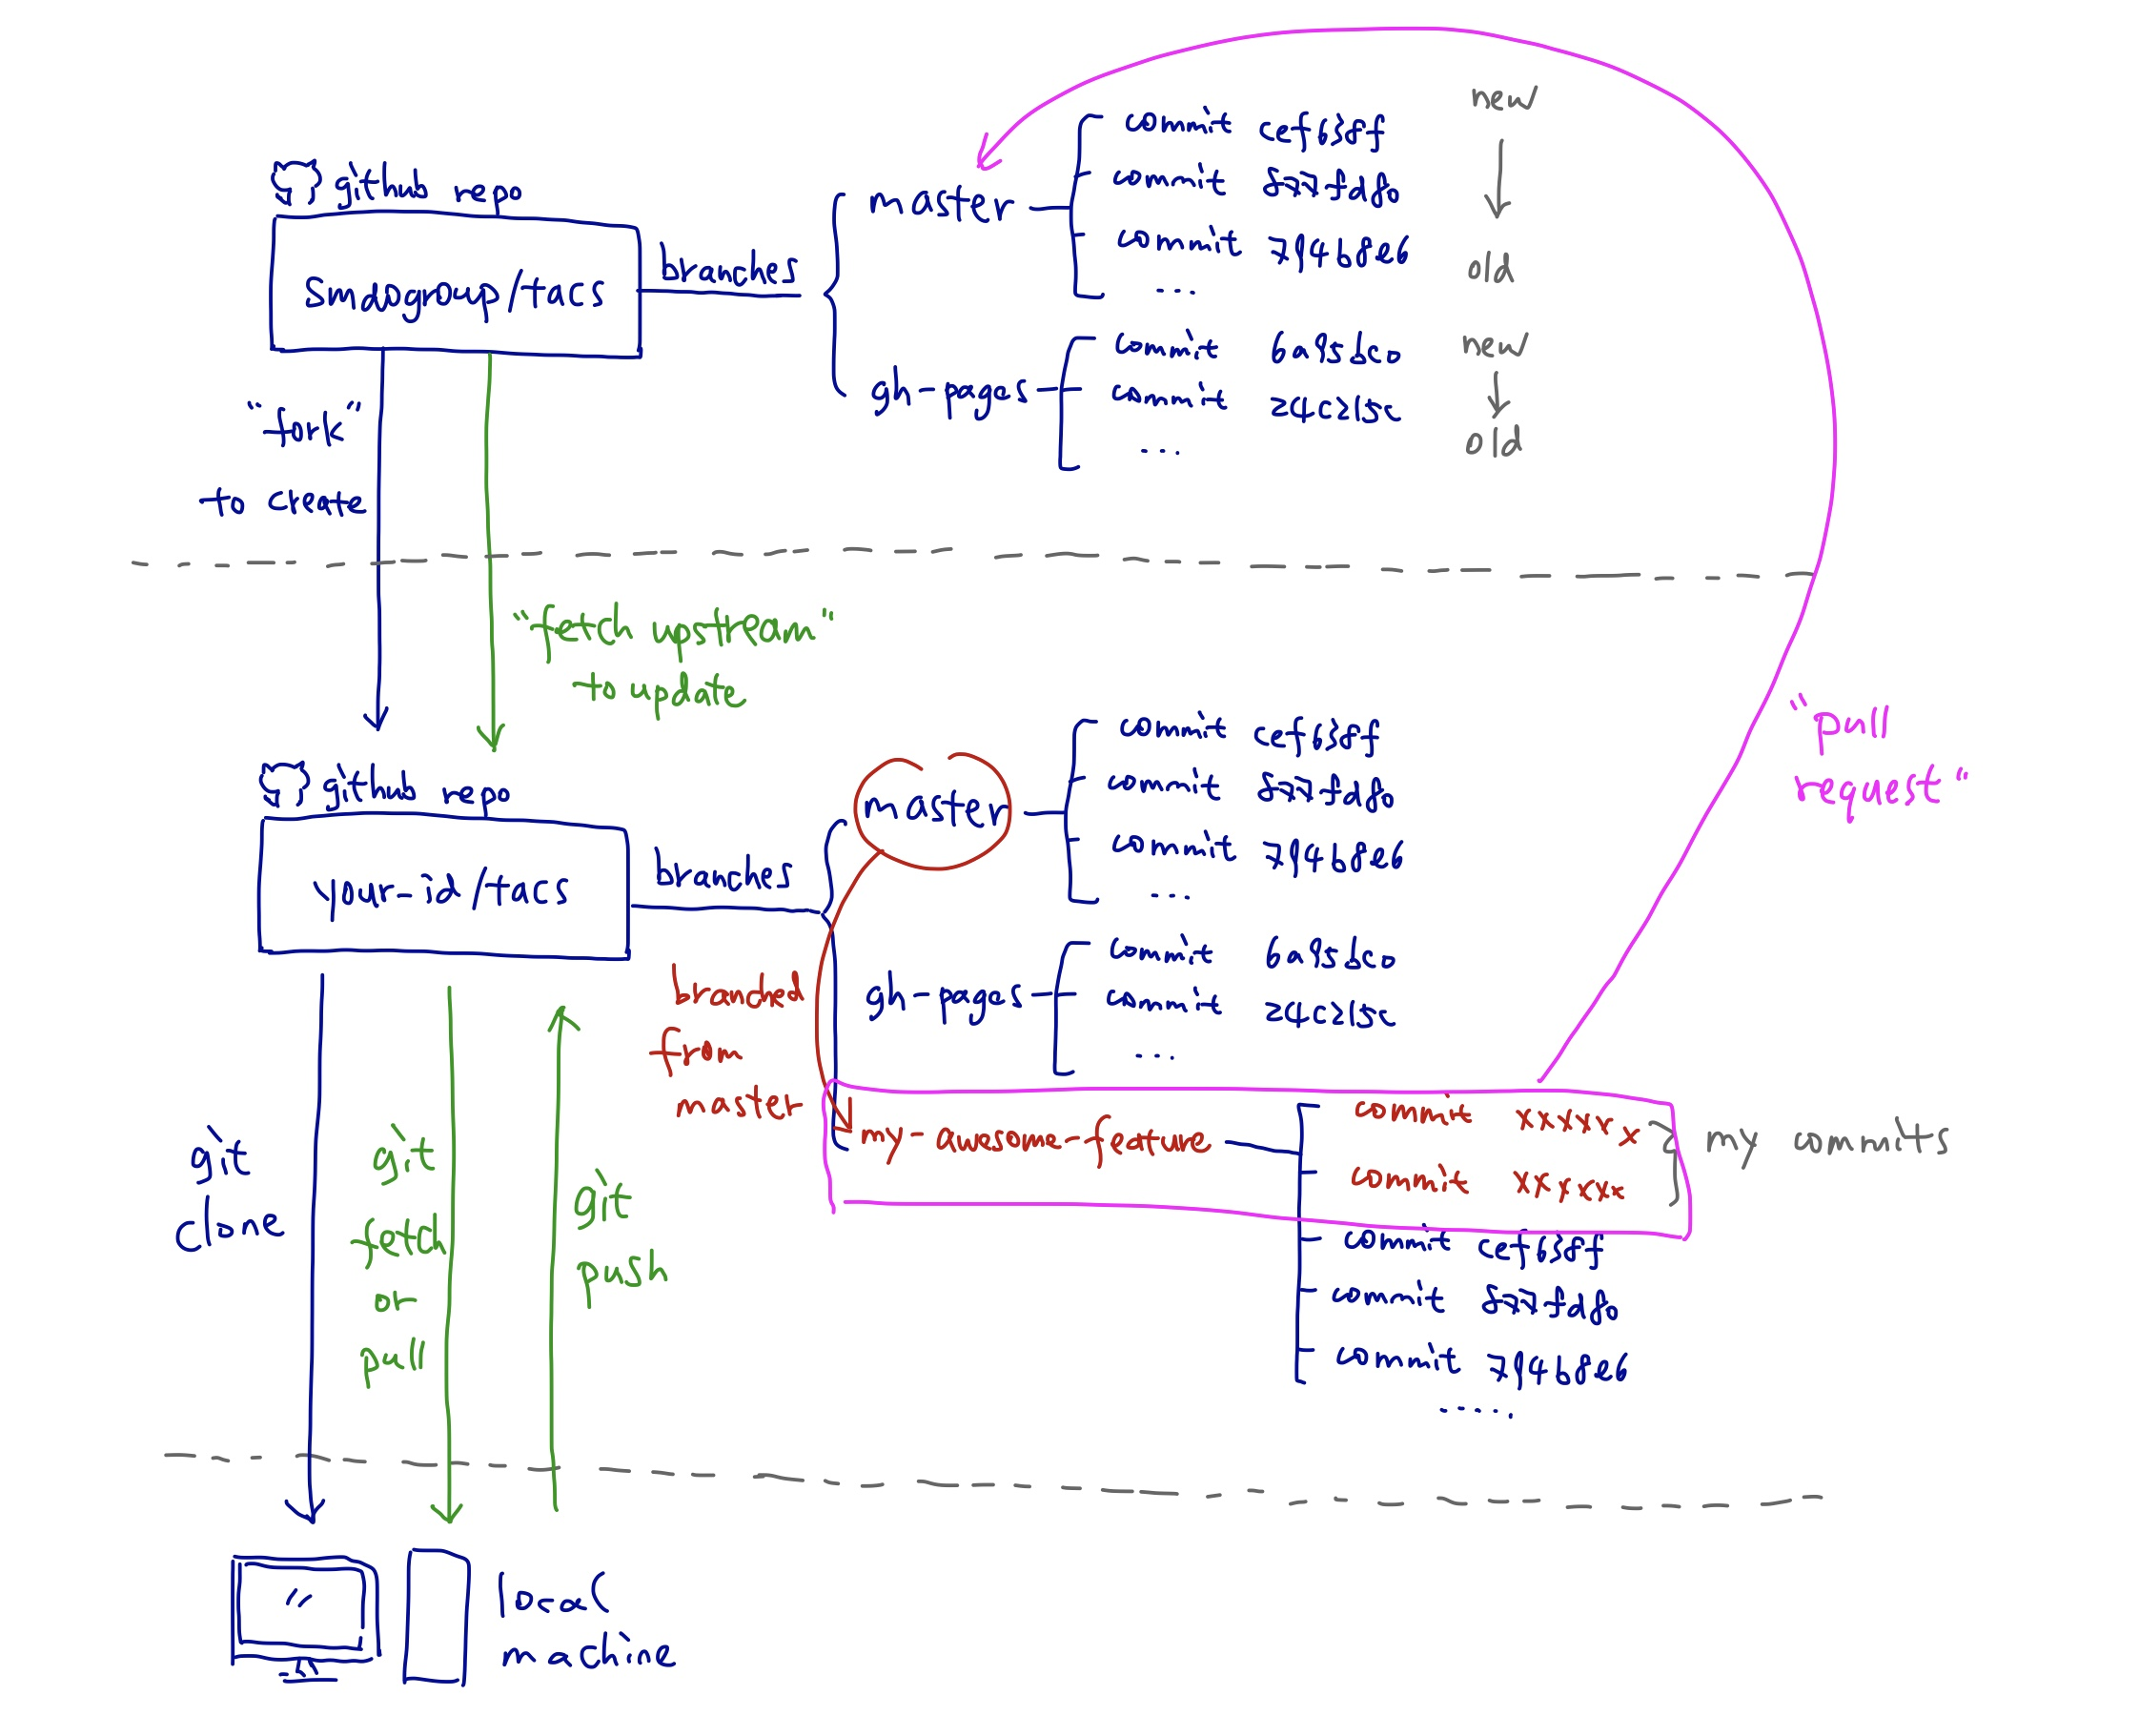
\includegraphics[width=0.9\textwidth]{pics/cartoon.jpg}
    \label{fig:cartoon}
    \caption{Git/github workflow diagram}
\end{figure}

The following is a step-by-step instruction:

\begin{enumerate}
    \item
    Go to group's GitHub page \href{https://github.com/smdogroup/}{https://github.com/smdogroup/},
    choose the repository you wish to work with, and click ``fork'' button to the upper right.
    This will create a separate repository under your own account.

    \item
    Clone the forked repo to your local machine.
    Notice that ``fork'' is a GitHub specific feature which git doesn't have.
    So once you clone the repo, anything you do with \texttt{git} command will only
    affect your ``forked'' repo, but not the ``upstream'' repo under smdogroup's account.
    This can be verified by running:

    \texttt{git remote --verbose}

    And you will only see the urls of your own remote repo (but not the repo under smdogroup).

    \item
    Create a new branch under your repo for the certain feature you'll be working on.
    The name of the branch should be precise and self-explanatory.
    This could be done either on the GitHub webpage, or locally by running the
    following command \textbf{on the branch you're branching from (for example master)}:

    \texttt{git checkout -b name-of-your-branch}

    which will create a new branch and switch to it.
    Then you can do:

    \texttt{git branch}

    to verify that you're at the right branch you want to be.

    Note:
    Branching is implemented in a very cheap way for git, and it makes the code base organized
    if many different features are developed at the same time.
    so it's a good practice to always make a branch for certain task.
    Never directly commit to the code to master (or main, which is GitHub's new nomenclature)
    branch, even for your own forked repo.

    \item
    Now you're ready to work on the code!
    you can commit as many times as you want to your branch.
    \texttt{git add}, \texttt{git commit}, \texttt{git pull} and \texttt{git push} will be your
    best friends for this.
    It's recommended to frequently push local changes to GitHub, such that you will always
    have fresh backups online.
    You can only push commits (but not uncommitted changes) so make sure to commit before push.
    Anytime you want to push local changes, make sure to \texttt{git pull} before \texttt{git push}
    in cases there are new changes in the remote repo you don't have locally.

    \item
    While we are working on the local fork, the upstream repo might change.
    So you need to periodically update your local fork.
    This needs to be done on the GitHub webpage, by simply clicking the ``Fetch upstream'' button.
    If there are indeed updates from upstream, you might also need to update your branch.
    This is because your branch was originated from some other branch (likely to be master),
    which might be updated by such action.
    You can update your branch by:

    \texttt{git checkout name-of-your-branch \&\& git merge branch-to-update-from}

    \item
    Once you feel comfortable with your changes, it's time for the main repo to incorporate your
    contributions!
    This will be done via ``pull request'', which is another GitHub specific feature that git doesn't
    have. So you will need to go to the GitHub webpage and open a pull request ticket.

    The name of pull request might be confusing, it means ``to request a pull to main from you".
    The pull request should be from your repo to smdogroup/repo, and usually it'll be to the master
    branch.
    The pull request then will be reviewed and tested and finally be approved and merged (hopefully).

    \item
    Once the pull request is approved, you should delete the local branch you've been working on.
    Never keep working on the merged branch and ``pull request'' again in the future,
    because it and will cause redundant commit history to the master branch.

    \item
    Lastly, you will do a final ``Fetch upstream'', then you're work will be reflected in the master
    branch of your own forked repo.
    And do another \texttt{git pull} locally to download the updates.

\end{enumerate}

Above is the workflow we would everyone in the group to follow.
This could be a little complicated if you never work with forking before.
But it will be beneficial for the main code base in terms of better organized (``squashed'')
update history and a cleaner list of branches in the main repo.

\end{document}
